% !TeX spellcheck = en_US
\section{Mobile Video Upload}
\label{sec:220_videoupload}

An essential step in the video streaming process (see Section~\ref{sec:210_streaming_process} and Figure~\ref{fig:205_relatedworkmbsstreaming}) is the live upload of a video stream from a smart mobile device.
The mechanisms that allow live upload to nearby or remote receivers are combined in a so-called \acf{MBS}.
In the remaining section, the \ac{MBS} is defined, and challenges in the scenario of mobile live video uploading are discussed. 
Finally, the existing \ac{MBS} approaches from both academia and industry are compared. 
\subsection{Description of an MBS}
The description of \ac{MBS} is derived from the \ac{PBS} as defined by the \ac{3GPP}~\cite{3GPP}.
The term \ac{MBS} is used in contrast to \ac{PBS} to emphasize the focus on mobile devices that provide live video.
A \ac{PBS} allows providing any media from any device.

An \ac{MBS} leverages smart mobile devices capable of recording and uploading video, i.e., broadcast or multicast them to a large set of receiving users. 
In the case of live broadcast, the video needs to be delivered to multiple users simultaneously.
The technical implementation of a broadcast is not described by the \ac{3GPP}, allowing it to be implemented on any suitable layer of the \ac{ISO}/\ac{OSI} network stack.
For the collection and the distribution of video streams, the \ac{MBS} uses network technologies supporting \ac{IP}.

Different roles exist in an \ac{MBS}.
The \ac{MBS} provider is an individual generating a video stream to distribute it to other users. 
In the remaining thesis, this role is replaced by the terms \emph{recorder} or \emph{recording user}.
The \ac{MBS} user consumes the media stream received from a recorder.
A consumer can be any device, but is assumed to be another smart mobile device. % or a server ranging from smartphones to \ac{IP}-connected displays.
In the remaining thesis, the \ac{MBS} user is called a viewer.
\ac{MBS}s may include independent service providers, such as Facebook, which offer servers to coordinate recorders and viewers. 
A service provider is responsible for the media delivery between the recorders and the receivers, possibly involving intermediate servers for processing.
In many cases, the involvement of such an intermediate service provider is not required. % they are not discussed in detail in this work
In the remaining work, service provider is represented by a server.
\subsection{Scenarios for Mobile Broadcasting Services}
\label{sec:220_Scenario}
Scenarios for \ac{MBS}s consist of the remote, the in situ, and the hybrid streaming (see Figure~\ref{fig:520_Scenario_Streaming}).
All scenarios take place with no dedicated network infrastructure for the \ac{MBS}; rather, they share networks with other applications and devices.
\begin{figure}[htb]
	\centering
	\subfloat[Remote Streaming]{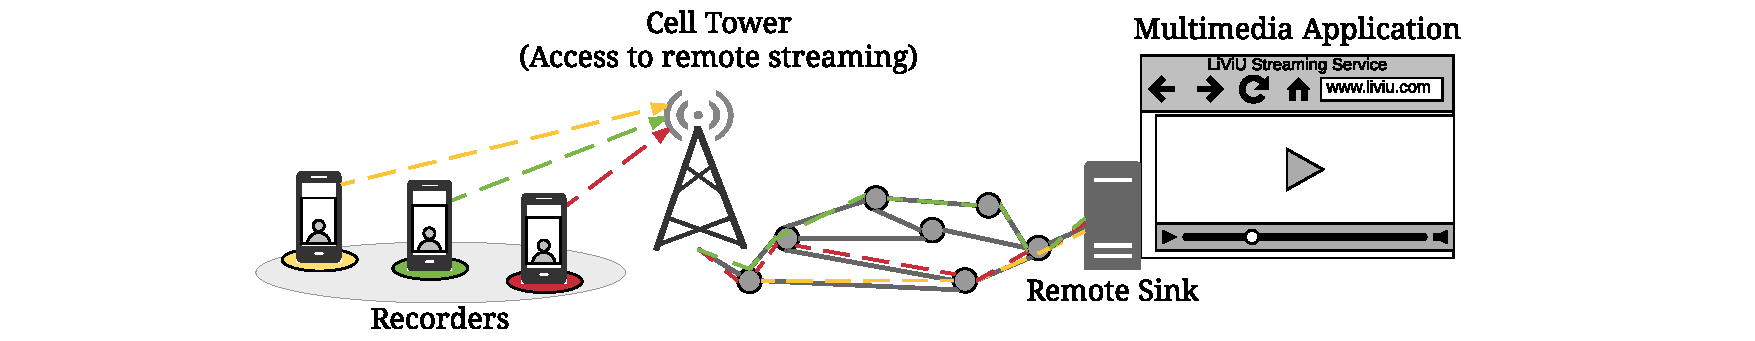
\includegraphics[width=\linewidth]{./gfx/500_MobileUpload/Scenario_Remote_Streaming}}\\
	\subfloat[In Situ Streaming]{
\includegraphics[width=\linewidth]{./gfx/500_MobileUpload/Scenario_InSitu_Streaming}}\\
	\subfloat[In Situ Streaming]{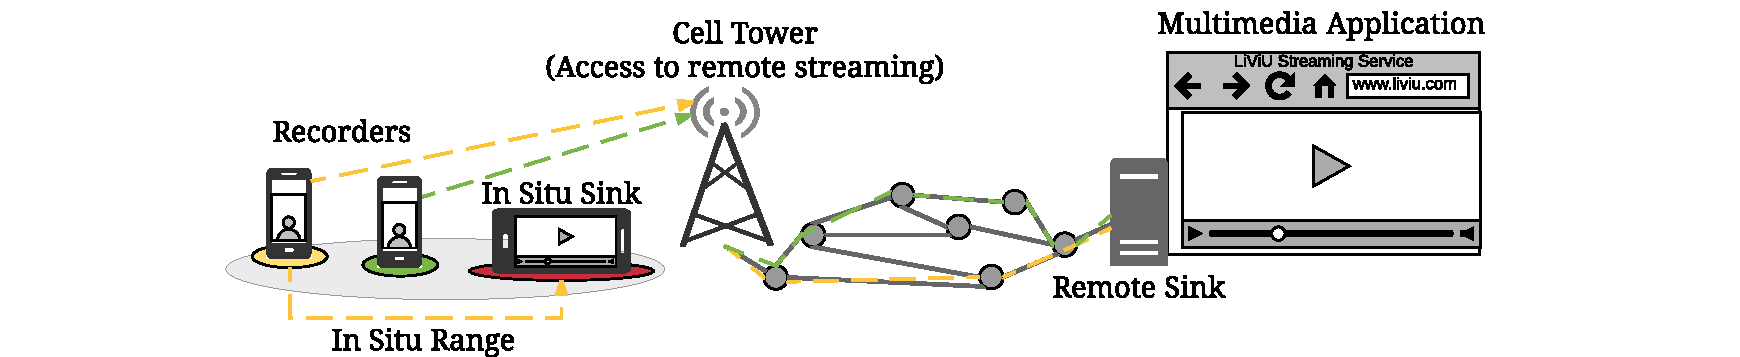
\includegraphics[width=\linewidth]{./gfx/500_MobileUpload/Scenario_Hybrid_Streaming}}
	\caption[Overview of Mobile Broadcasting Services]{Overview of the MBS scenarios discussed in this thesis.}
	\label{fig:520_Scenario_Streaming}
\end{figure}
\subsection{Remote Streaming}
The remote streaming scenario consists of two roles: the recorder and the receiver (or server) of a video stream.
Any distance can be between the recorder and the server, but an \ac{IP}-based network connects both.
In this scenario, the focus lies on the nearly ubiquitously available cellular networks. 
Their available resources are limited.
\ac{LTE}, for instance, achieves an average of $9.86\unit{\frac{MBit}{s}}$ in 2015 in the United States of America~\cite{OpenSignal2016}.
\ac{UMTS} connections achieve in the same year and region an average throughput of $1.75\unit{\frac{MBit}{s}}$~\cite{OpenSignal2016}. 
Upload speeds of end user Internet connections are lower, as they are asynchronously configured in relation to the download speed.
\ac{LTE} achieves upload speeds of up to $75\unit{\frac{MBit}{s}}$ when the setup supports $300\unit{\frac{MBit}{s}}$ on the downlink at $20$ $\unit{Mhz}$~\cite{Ghosh2010}. 
Empirical studies by Shah et al. report for 2016 that the upload speeds are very different depending on the geo-location~\cite{Shah2016}.
Whereas in North America upload speeds of up to $23\unit{\frac{MBit}{s}}$ could be achieved, the speeds in India and Pakistan ranged from $300$ to $600\unit{\frac{KBit}{s}}$ and in South America from $200$ to $300\unit{\frac{KBit}{s}}$.
The latency of the connections in cellular networks are in average below $150$ milliseconds, and thus not critical for the remote streaming scenario~\cite{OpenSignal2016}.

This thesis discusses scenarios where the movement speed is limited to pedestrian walking speeds. Thus, transmissions during vehicular movements are not in the focus\footnote{The evaluation in Chapter~\ref{sec:700_VAS} shows that our contributions reliably work at vehicular speeds.}.
These speeds usually have only a slight impact on the available throughput in cellular networks.
Thus, in the remote streaming scenario, mobility plays a minor role, as cellular networks shows a comparably high coverage (up to 86.73\%~\cite{OpenSignal2016}) in developed countries, and automatic handover mechanisms exist, which guarantee a low probability of connection losses.
This scenario is throughput-constrained, and rather insensitive to pedestrian mobility and latencies.
\subsection{In Situ Streaming}
\label{sec:520_scenario_insitu}
%Low Delay
An in situ scenario consists of at least one recording device and one receiving device in close proximity to each other.
This distance should be less than the communication range of the wireless network technology in use.
As a communication network, IEEE 802.11 is assumed to be used.
Whereas in a remote streaming scenario an initial hop has to be made to access the core network via a cellular network tower (\ac{LTE} or \ac{UMTS}), a regional distribution of the video is intended in the in situ streaming.

As the receivers are in close distance of each other, the focus lies on low-delay streaming.
Ideally, a user receiving a video stream should not notice any delay between a live performance and the recording played back on a mobile device.
In comparison to the remote streaming case, a single device may distribute the video to more than one receiver.
A specific challenge in this scenario is the mobility of the devices. 
It does not necessarily lead to varying throughput conditions.
But, if the devices move, the sender and receivers may leave the communication range.
A direct communication in a single-hop communication pattern may no longer be possible. 
In these cases, other devices in the range of both sending and receiving devices
help to establish and maintain communication.
\subsection{Hybrid Streaming}
In a hybrid scenario, mobile recorders stream media to nearby receivers as well as to a remote streaming sink, e.g., a server.
Until now, no \ac{MBS} has been proposed which addresses this hybrid scenario.
One reason is the challenge to combine low-delay in situ streaming with a high-quality, bandwidth-constrained remote streaming.

In a hybrid streaming scenario, a single network interface may not reach all the intended receivers of a media stream.
Another engineering challenge may thus be multiple network interfaces, i.e., IEEE 802.11-based and cellular networks.
Appropriate \ac{MBS} protocols are required for an efficient transmission of the media streams. 
\subsection{Existing Work on MBSs}
\subsubsection{Categorizing MBSs}
We now classify existing work on \ac{MBS}s.
The discussion focuses on assessing the abilities to cope with varying network conditions, to leverage content adaptation, and whether a prototype of the \ac{MBS} was developed.

The live streaming support is essential for an \ac{MBS} so that each evaluated proposal is classified regarding the live streaming support (LS).
A live streaming support can be at the heart of a protocol (+), be supported ($\circ$) or not discussed (-). 
The scenarios (S) introduced in Section~\ref{sec:220_Scenario} needs to be supported by an \ac{MBS}.
Scenarios range from remote (R), in situ (I) to hybrid streaming (H).

Related to the streaming scenario is the classification of different \ac{MBS} applications with respect to the supported network technologies (NW). Either IEEE 802.11 or cellular networks such as \ac{LTE} or \ac{3G} networks are used. 
Furthermore, the support for ad-hoc streaming is denoted by "A". 

Mobile support (M) describes the characteristic that a proposed \ac{MBS} makes assumptions which do not hold for smart mobile devices.
If mobile support is not provided, no working prototype of the system can be built on retail phones (-).
An existing prototype or a simulative model, which can be mapped to a prototype supports this characteristic (+).

In any of the described networking scenarios, a common phenomenon is the uncertainty about the network conditions, which includes varying delays and throughput rates.
Content adaptation in the form of adaptive video streaming (AS) is a promising solution to the challenges.
If a proposed \ac{MBS} uses an adaptive streaming approach and realizes it on a smart mobile device, it is perceived as supporting this feature (+).
Theoretical approaches that cannot be realized with existing technology are described by a $\circ$ in our classification.
A system without support for adaptive streaming is described with a -.

How media streams are distributed can be classified into push-based (P) delivery, where the recorder sends the media stream to the viewers,
or pull-based delivery in which the viewer requests the media stream (PL).
The type of distribution is termed scheduling (SCH).

Besides media streams, mobile recording devices contain a broad range of sensors, which can be used to understand the context of a recording. The auxiliary data support (ADS) of each protocol is evaluated.
A protocol can support auxiliary data including monitoring data, or sensor samples (+) or not (-).

The next two characteristics indicate if the proposed methods have lead to a real prototypical evaluation (Pr) of the system, and if standardized protocols 
(SP) are used for the design of the \ac{MBS}.
SP represents a list of the used transmission protocols.

Limited throughput rates are a major, but common challenge for \ac{MBS}s.
We evaluate the different prototypes, if they can cope with challenged network conditions such as limited upload capacities (LMU).
We distinguish, if a proposed system addresses changing and poor network conditions (+) or not (-) in the protocol design.

Another challenge is the streaming delay (DS), which is critical in the in situ streaming scenario and still essential in remote streaming scenarios.
It is distinguished, if the protocol does (+) or does not consider the streaming delay (-).

The proposed upload protocols are used by multimedia applications.
The last characteristic describes, if the protocol supports specifications and requirements of the multimedia applications (MAR).
It is distinguished if a protocol does not support (-), can in general support requirements of the application ($\circ$), or can adapt to requirement during a session (+).
\subsubsection{Comparison of MBSs}
\label{sec:220_existing_mbs}
Table~\ref{tab:220_Related_Work} gives an overview of existing \ac{MBS}s and gives a comparison of the systems regarding the discussed characteristics. 
\begin{table}
	\centering
	\caption[Discussion of related work on MBS]{Overview of related work for \acf{MBS}. Features used for comparison include LS: live streaming support; S: Scenario; NW: network access technology; M: mobility awareness; AS: adaptive streaming support; SCH: scheduling; ADS: auxiliary data support; Pr: prototype available; SP: list of standardized protocols used; LMU: limited upload capacity; DS: delay sensitive. MAR: multimedia application requirements support. +: implemented; $\circ$: compatible; - unsupported;}
	\begin{tabular}{lcccccccccccc}
		\toprule[1.5pt]
		&  \textbf{LS} &\textbf{S} & \textbf{NW} & \textbf{M} & \textbf{AS} &\textbf{SCH} &\textbf{ADS} &\textbf{Pr} &\textbf{SP}&\textbf{LMU} &\textbf{DS} &\textbf{MAR} \\ 
		\toprule[1.5pt]
	$ \left.\begin{array}{l} \mbox{Twitch.tv~\cite{Zhang2015}}\\\mbox{YouNow~\cite{Stohr2015}}\\\mbox{Periscope~\cite{Siekkinen2016}}\\\mbox{Facebook.Live} \end{array} \right\}$	&+  & R & 802.11,3G+& -	& - & P &  $\circ$  & + &  RTMP & - & $\circ$ & $\circ$\\ \hline
	NEWSMAN~\cite{Shah2016} 	& - & R &(802.11,3G)& + & $\circ$ & P &-  & - & - & + &- & -\\ % Delay nicht diskutiert / Adaptierbarkeit nein
	DMUS~\cite{Zhang2008}	 	& - & R & - 		& - &  -  & P &-  & - & - & + &- &-\\ % Delay nicht diskutiert / Adaptierbarkeit nein
	DASH-POST~\cite{Seo2012} 	& + & R & 802.11 	& + &  $\circ$ & P &-  & + & HTTP &- & +&-\\ % Delay diskutiert / Adaptierbarkeit nei
	ASMA\cite{MinQin2010}		& + & I & 802.11,A	& + & + & P   & -  & - & - &+ &- &-\\
	CoStream~\cite{Dezfuli2012,Dezfuli2013}	& +  &I & 3G  		& +  & - & P   & -  & +  & RTP & -& +& -\\
	\cite{Siekkinen2016}& + & R & 	-	& - & $\circ$ & P & -  & - & HTTP & + &- &+\\
	MoviSode~\cite{Seshadri2015}& - &R&3G,802.11& + &- & P  & + & + & - &- &- &+\\
	MediaQ~\cite{Kim2014}		& $\circ$ &R &- 	& + &-  & P & + & + &- &- &- &- \\
	SODiCS~\cite{Ito2014}		& + & R & 802.11& + &-  & PL & + & + & - & - & - & -\\
	\cite{ElEssaili2015}	& + & R & LTE	&-  & $\circ$ & P & - & - & - & +& -& -\\
	DAVII~\cite{Johansen2009}	& + & R & -		& + & + & P & + & + & HTTP & + & - & $\circ$ \\
	\cite{Richerzhagen2016}	& + & R,(I)& 802.11,A & - & $\circ$ & P  & + & - & -& + & -& +\\
	\bottomrule[1.5pt]
	\end{tabular} 
	\label{tab:220_Related_Work}
\end{table}

\paragraph{Industry Solutions}
The most widely used protocol for efficient media streaming is the \ac{RTMP}.
The protocol relies on the \ac{TCP} and thus ensures in-order and error-compensated transmission of messages.
It is thus a stateful media streaming protocol, which is message-oriented. 
\ac{RTMP} establishes a reliable, low-delay end-to-end connection between a mobile device recording a digital video and a server. 
A streaming session is established using a three-way handshake procedure, which exchanges authentication information of both the recorder and the receiver. 
The rather complex handshake procedure is depicted in Figure~\ref{fig:220_RTMP_Handshake}.
\ac{RTMP} establishes a secure application layer coordination to ensure, that sender and receiver of a media stream use the same protocol version.
Random bytes are sent to test the network connection and make an initial guess of the best fragment size.
The fragment size determines the maximum payload of a media message.
It shall ensure proper live streaming, without congesting the network or receiver.
\begin{figure}[htb]
	\centering
	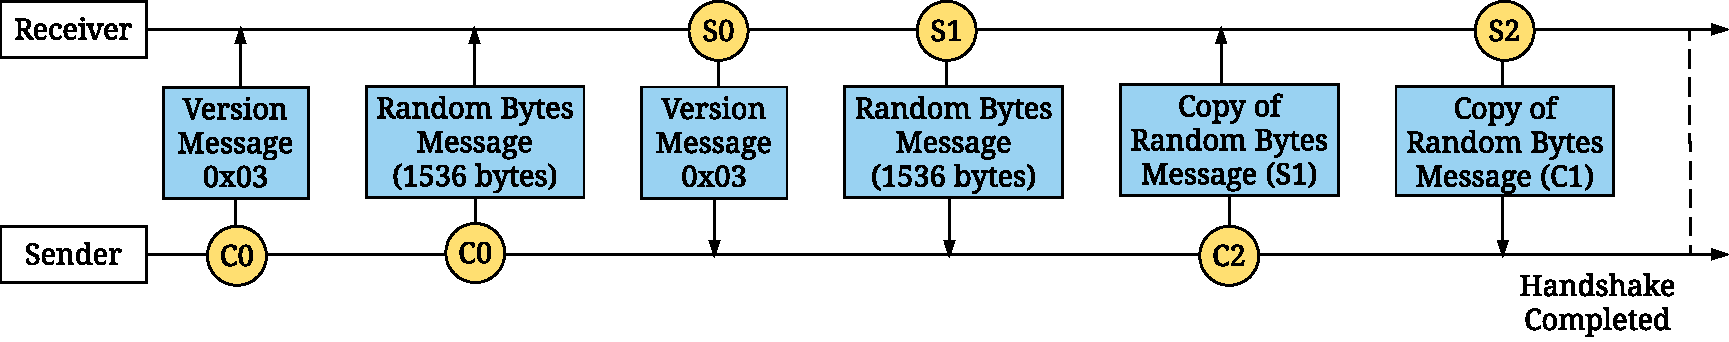
\includegraphics[width=\linewidth]{./gfx/500_MobileUpload/RTMP_Messages}
	\caption[Joining procedure of the protocol RTMP]{Joining procedure of the protocol RTMP~\cite{RTMP2009}.}
	\label{fig:220_RTMP_Handshake}
\end{figure}
\ac{RTMP} is able to transfer multiple synchronized audio and video tracks in parallel.
An established connection is able to transmit media segments of variable lengths with a compressed header and thus reduces the overhead.
As a consequence of the join procedure, \ac{RTMP} requires a rather long time until a connection is ready for media stream transmissions.
Today, \ac{MBS}s are required which contain a join procedure that does not delay the transmission of initial video segments. 
An advantage of the protocol is the message structure when a connection is established.
Header overhead is minimized as long as the connection exists. 

Twitch.tv~\cite{Zhang2015}, YouNow~\cite{Stohr2015}, Periscope~\cite{Siekkinen2016}, and Facebook.Live use \ac{RTMP} as a streaming protocol, and add HTTP for the transmission of auxiliary data such as network metrics or \ac{GPS} coordinates.
None of the approaches supports in-time adaptive streaming.
The design of \ac{RTMP} allows a delay to be kept low during a streaming session but the initial joining procedure is time-consuming.
The system does not support any mechanisms to cope with very low upload rates. 
For Periscope, it is reported, that due to the streaming setup a minimum of $2 \unit{\frac{MBit}{s}}$ is needed for a stall-free upload~\cite{Siekkinen2016}.
\paragraph{Mobile Video Upload}
Besides \ac{RTMP}, new research prototypes have risen to compensate for weaknesses of the reliable, but rather static standard.
NEWSMAN allows the upload of news videos from mobile devices~\cite{Shah2016}.
It does not aim for live streaming in the classical sense as middleboxes are introduced, which decouple transmission to the middleboxes from the long-haul transfer to remote servers.
It optimizes the scheduling of the videos created by the recorders and selects an appropriate video quality for each recording.
Quality selection and transcoding are performed on the middleboxes.
A simulative study without a modeled underlying network was performed to evaluate the transcoding and scheduling of the videos.
Besides NEWSMAN, a range of similar protocols exist, which do not focus on the immediate, but the delay-tolerant distribution of video streams recorded on a mobile device.
One example is DMUS by Zhang et al.~\cite{Zhang2008}.
\paragraph{Support for Auxiliary Data}
MoviSode does not offer live upload of video streams, but was one of the first systems to introduce auxiliary data upload~\cite{Seshadri2015}. 
% besides the video itself.
The application allows video streams to be annotated with the \ac{PoI} coordinates. 
Remote users can query for the \ac{PoI} and retrieve a list of devices offering the respective video streams.
The list determines the priority of the video streams being uploaded.
A similar approach is pursued by Kim et al. with MediaQ, a multimedia collection and management framework~\cite{Kim2014}.
The proposed mobile application uses a sensor to describe when, where, and what has been recorded including the detection of \ac{PoI}s.
The focus of neither MediaQ nor MoviSode lies on the efficient upload in challenged networks. 
Thus, aspects such as adaptive streaming support or flexible scheduling are not discussed. 

SODiCS can collect video in a pull-based manner from mobile devices~\cite{Ito2014}. 
The basic idea is that videos and sensor data are gathered and stored by servers or cloudlets.
Mobile cameras always try to save their videos on the remote server.
It copes well with any breakdown of a cellular network. % to the local server in a push-based manner.  
\paragraph{Adaptive Live Uploading}
Media upload protocols can learn from the distribution protocols for video streams.
Thus, Seo et al. discuss how the \ac{MPEG} \ac{DASH} standard can be applied to media upload~\cite{Seo2012}. 
For this purpose, they leverage the \ac{HTTP} POST method to upload a segmented video stream to a server.
The proposed \ac{MBS} uses a server-driven adaptation and transcoding scheme and achieves a start-up delay of about the duration of one video segment in \ac{WLAN}s.

Siekkinen et al. extend the idea of using \ac{DASH} by using an \ac{MVLC} for allowing adapting video content to the upload conditions~\cite{Siekkinen2016}.
As no prototypical real-time production of \ac{MVLC} is possible, the proposed scheduling strategies are evaluated in simulations.
No validated wireless channel model has been used to model the upload, but the proposed SVC-DASH shows that an optimal selection of the bit rate of each video chunk improves the continuity and the overall quality of video streams. 

El Essaili et al. investigated the process of uploading a video when a central entity can coordinate the scheduling of transmissions in an \ac{LTE} network~\cite{ElEssaili2015}.
The system is described as QoE-UL for its ability to support quality-driven uploads.
They show an optimal decision for the uplink transmission and determine which client should upload the video at what point in time. 
They optimize the resource usage and offer both low complexity as well as optimal scheduling strategies.
Additionally, a centralized approach allows multi-device and cross-layer optimization.
Their system is based on a significant number of requirements that cannot hold in a real deployment. 
For example, mobile devices are assumed to leverage \ac{MVLC}s which is not possible in real-time.
Additionally, the assumption that current \ac{MVLC}s result in less data traffic in comparison to non-scalable encoding has shown to be incorrect for current standards~\cite{Grafl2013}.

The DAVVI system is designed to generate video segments and upload them immediately after recording in order to generate a low-delay video streaming experience~\cite{Johansen2009}. 
Johansen et al. report how they dynamically adapt the bit rate of a video during the upload, which is achieved using a middlebox server for transcoding and segmenting.
Also, DAVVI allows the distribution of metadata and uses \ac{HTTP} for media upload.
\paragraph{In Situ Streaming}
The idea of in situ streaming is driven by CoStream~\cite{Dezfuli2013,Dezfuli2012}.
Their work describes beneficial \ac{UI} design and collaboration styles when using an \ac{MBS}.
Their research supports the easy retrieval of media streams shared by a group in a live streaming manner.
The system leverages a nearby server that mediates the streams between recorders and viewers. 
The upload is conducted in a push-based manner using the \ac{RTP}, achieving upload delays of around one second.

An in situ streaming scenario is used by \ac{ASMA}, which focuses on the optimal push-based scheduling of video streams encoded in different video layers using an \ac{MVLC}.
The method assumes that \ac{MVLC} can be efficiently produced on a mobile device. This work specifically addresses varying network conditions using adaptive streaming.
Specific features of IEEE 802.11 in ad-hoc mode are used to support the probabilistic scheduling and layer selection process.

A simulative model for a collaborative upload of video streams produced by phones is proposed by Richerzhagen et al.~\cite{Richerzhagen2016}.
The system leverages multiple network interfaces to share video streams in situ and with remote receivers.
The in situ distribution is used so that each device can act as a relay for accessing remote servers when no cellular connection is available.
The simulation assumes that video streams are efficiently produced as an \ac{MVLC}, which is not possible on smart mobile devices till today.

\subsection{Discussion}
A set of protocols exists that supports live upload of digital video.
Only a few systems exist that cope with changing network conditions by integrating content adaptation (adaptive streaming support). 
Also, most of the proposed protocols do not address how to cope with varying application requirements and are specifically designed for a single multimedia application.
The combination of content adaptation and a feature to react to application requirements promises to be beneficial for an \ac{MBS} in order to cope with both limited upload capacities (LMU) but also delay-sensitive applications (DS).
Most of the existing \ac{MBS}s focus on a push-based scheduling and neglect the advantages of a receiver pulling video stream segments, as, e.g., proposed by SoDiCS.

Also, modern protocols for \ac{MBS}s must support the transport of auxiliary data to annotate media streams with context information.
Only a small set of existing protocols is capable of transmitting this data.

In summary, there is a lack of an \ac{MBS} - supporting mechanisms to cope with varying network conditions - that aims for a low-delay, high-quality streaming experience and addresses the requirements of multimedia applications (auxiliary data, adaptive video streaming and scheduling).